
\section{Exercises}

\begin{exercise}
 \label{ex:03-power-euler} 
Prove that the power of the circumcircle with with respect to the common center in each of the following 3-periodic families is constant and given by the listed expressions. (i) incircle: $-a_e b_e$; (ii) homothetic: $-({a_e^2+b_e^2})/{2}$, and (iii) excentral: $-a^2-b^2-2\delta$. 
\end{exercise}

\begin{exercise}
\label{ex:03-cosine-circle}
Prove the radius $r^*$ of the stationary cosine circle of the excentral family is larger than the major axis $a$ of its caustic. 
\end{exercise}

\begin{exercise}
Prove \cref{lem:03-circum-x5-locus}.
\label{ex:03-circum-x5-locus}
\end{exercise}

\begin{exercise}
Derive the proof details to the 2nd part of \cref{prop:03-n3-role-reversal}.
\end{exercise}

\begin{figure}
    \centering
    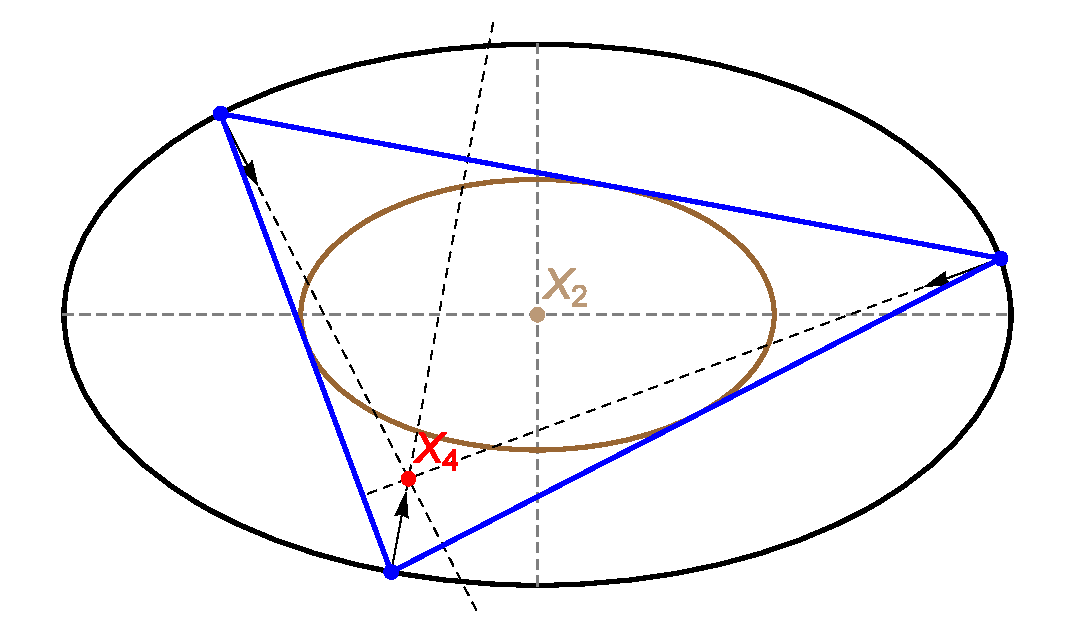
\includegraphics[width=.6\textwidth]{chap_03/pics/pics_03_280_homoth_x4.eps}
    \caption{Normals to the ellipse at vertices of 3-periodics in the homothetic family concur at the orthocenter $X_4$.}
    \label{fig:03-homoth-x4}
\end{figure}

\begin{exercise}
Prove that ellipse normals at vertices of 3-periodics in the homothetic family are concurrent at the orthocenter $X_4$, see \cref{fig:03-homoth-x4}. Derive the semi-axes of the elliptic locus of $X_4$ as a function of $a,b$ of the outer ellipse, see it \href{https://bit.ly/3fpESjh}{Live}.  
\label{ex:03-homoth-x4}
\end{exercise}

\begin{exercise}
The Thomson cubic (see \cref{que:03-thomson}) is the locus of centers of circumconics such that normals at the vertices concur (on the Darboux cubic); see \cite[Darboux and Thomson cubics]{gibert2021-ctc}. Prove that vertex normals off of the $X_1$- and $X_6$-centered circumconics concur on $X_{84}$ and $X_{64}$, respectively. This readily implies normals to the outer ellipse at the incircle and excentral family vertices will concur on said points; see \cref{tab:03-normal-concurrence}. 
\end{exercise}

\begin{table}
\centering
\begin{tabular}{|r|c|c|c|}
\hline
\makecell[rc]{Poncelet\\family} &
center &
\makecell[cc]{norms.\\concur} &
\makecell[cc]{concur\\ \texttt{bit.ly/*}} \\
\hline
incircle & $X_1$ & $X_{84}$ & \href{https://bit.ly/3eVuCQY&}{\texttt{3eVuCQY}} \\
homothetic & $X_2$ & $X_4$ & \href{https://bit.ly/3eXSRhC}{\texttt{3eXSRhC}} \\
circumcircle & $X_3$ & $X_3$ & \href{https://bit.ly/2RqMqul}{\texttt{2RqMqul}} \\
dual & $X_4$ & $X_{3346}$ & n/a \\
excentral & $X_6$ & $X_{64}$ & \href{https://bit.ly/3hwCTfN}{\texttt{3hwCTfN}}\\
confocal & $X_9$ & $X_1$ & \href{https://bit.ly/3uTvqLI}{\texttt{3uTvqLI}} \\
\hline
x57 & $X_{57}$ & $X_{3345}$ & n/a \\
\hline
\end{tabular}
\caption{CAP families studied herein. Coincidentally, their centers lie on the Thomson cubic  which is the loci of circumconic centers such that normals at vertices concur \cite[Thomson Cubic]{gibert2021-ctc}. The third column lists the experimentally-found concurrence points. These lie on the Darboux cubic \cite[Darboux cubic]{gibert2021-ctc}.}
\label{tab:03-normal-concurrence}
\end{table}

\begin{exercise}
Recall the dual family has stationary orthocenter $X_4$. Prove that the inversive image of the dual family wrt to a circle concentric with the ellipse pair is a non-Ponceletian family with incenter $X_1'$ stationary at the common center. This inversive family is inscribed in Booth's curve and its caustic can contain multiple spikes; see it \href{https://bit.ly/3vCCe05}{Live}.
\end{exercise}

\begin{exercise}
Given a reference triangle $T$, its tangential triangle $T'$ has sides tangent to the circumcircle at the vertices of $T$. A known fact is that the sides of $T'$ are parallel to those of the orthic $T_h$ of $T$, see \cite[Tangential Triangle]{mw}. For any acute triangle $T$, the Gergonne point $X_7'$ of the tangential triangle coincides with the symmedian $X_6$ of $T$, see \cite[Contact Triangle]{mw}.

Let $T$ denote the Poncelet family of excentral triangles. We've seen above that (i) this family is all acute, and that (ii) its symmedian point $X_6$ is stationary. Let $T'$ denote their tangential triangles. This family will be non-Ponceletian: its vertices do not sweep a conic nor do its sides envelop one.

Since the $T$ are all acute, they can be thought of as the contact triangles of the $T'$. Therefore the Gergonne point $X_7'$ of the tangentials to the excentrals will coincide with $X_6$ of the excentrals and be stationary, see \cite[Contact Triangle]{mw}.

Prove that the ratio of homothety between the orthics (billiard 3-periodics) and the tangentials is invariant. Corollaries: (i) the $T'$ conserve perimeter; (ii) they conserve the same $r/R$ as the excentral orthics, i.e., the corresponding billiard 3-periodics. See it \href{https://bit.ly/3o7JM8V}{Live}.

Also prove that the locus of $X_9'$ of the $T'$ is an ellipse.

Derive equations for the curves swept by the vertices of $T'$ as well as their caustic. 
\end{exercise}